\documentclass{article}

% if you need to pass options to natbib, use, e.g.:
\PassOptionsToPackage{numbers, compress}{natbib}
% before loading nips_2017
%
% to avoid loading the natbib package, add option nonatbib:
% \usepackage[nonatbib]{nips_2017}

\usepackage[final]{nips_2017}

% to compile a camera-ready version, add the [final] option, e.g.:
% \usepackage[final]{nips_2017}

\usepackage[utf8]{inputenc} % allow utf-8 input
\usepackage[T1]{fontenc}    % use 8-bit T1 fonts
\usepackage{hyperref}       % hyperlinks
\usepackage{url}            % simple URL typesetting
\usepackage{booktabs}       % professional-quality tables
\usepackage{amsfonts}       % blackboard math symbols
\usepackage{nicefrac}       % compact symbols for 1/2, etc.
\usepackage{microtype}      % microtypography
\usepackage{amsmath}
\usepackage{graphicx}
\usepackage{grffile}

\newtheorem{prop}{Proposition}

\title{Second Order Momentum}

\author{
  Vaibhav Sinha \\
  \texttt{cs15btech11034@iith.ac.in}
  \And
  Sukrut Rao \\
  \texttt{cs15btech11036@iith.ac.in}
}

\begin{document}

\maketitle

\begin{abstract}
  We study the effect of momentum on two second order methods - Newton's method and BFGS. We empirically determine the performance as compared to gradient descent, with and without momentum, as well as Cubic Regularization. For applying momentum, we consider both the classical momentum and Nesterov's accelerated gradient.
\end{abstract}

\section{Objective and Introduction}\label{introduction}

To achieve faster convergence, second order methods were proposed over first order methods. Although second order methods have better theoretical bounds than first order methods and converge in very few steps, they are often not used in practice due to the cost of each step. To cope with these problems, two approaches have been proposed and well studied: (i) Adding momentum \cite{POLYAK19641,Sutskever} to first order methods to make the convergence speed comparable to second order methods, (ii) Quasi-Newton methods \citep{davidon,broyden1965class,nocedal1980updating} which avoid the costly computations involved in second order methods, with a small cost on the rate of convergence. In this project, we aim to combine both these approaches and attempt to verify if the classical second order methods as well as Quasi-Newton methods can be accelerated.

Momentum has been extensively studied on first order methods \citep{POLYAK19641,Sutskever}. However, there seems to be almost no work done on the effects of momentum on Newton’s method. Through this project we seek to address this problem. <Write about that paper>.

We apply momentum to two methods - Newton's method and BFGS. We use both the classical momentum proposed by [] and Nesterov's accelerated gradient proposed by \citet{Sutskever}. A comparison of these approaches is made with gradient descent, gradient descent with momentum, and for some functions, with Cubic Regularization. We study the convergence rates empirically for five convex and five non-convex functions, mostly taken from various benchmarks.

The report is organized as follows. Section \ref{momentum} describes the two momentum methods and their update formulae. In Section \ref{methodology}, we describe our extension of the formulation of momentum for second order methods. Then, in Section \ref{opt}, we describe the methods used for optimization, such as gradient descent and BFGS. This is followed by description of the methods used for finding step sizes in Section \ref{step}. We list the functions used to empirically test our approach in Section \ref{functions}. The experiments conducted then follow in Section \ref{experiments}, and their results are described in Section \ref{results}. Based on these results, we provide our inferences subsequently in Section \ref{inferences}, and conclude in Section \ref{conclusion}.

The code used in this project can be found in its GitHub repository at \url{https://github.com/vbsinha/Second-Order-Momentum}.

\section{Momentum}\label{momentum}

The objective of momentum methods is to accelerate the descent towards the optimal value. It 'damps' the gradient descent when close to the optimal, that allows the use of higher learning rates while avoiding overshooting the point of minimum.

Momentum was first proposed by [] in []. Subsequently, in 2013, usage of Nesterov's accelerated gradient for deep learning was proposed by \citet{Sutskever}, which gave good empirical results.

The update step for gradient descent is given by
\begin{equation}
x^+ = x - \eta \nabla f(x)
\end{equation}

In general, with an optimization method that updates by $U$, the update step is given by
\begin{equation}
x^+ = x - \eta U
\end{equation}

With momentum, this update step is modified to include a velocity term, and the update depends on the relative weights given to the velocity direction and the descent direction, parameterized by a momentum parameter $\gamma$.

\subsection{Classical Momentum}
In this method, we introduce a velocity $v$, which is initialized with $0$. Then, the update step is given by
\begin{align}
v^+ &= \gamma v + (1-\gamma) \nabla f(x) \\
x^+ &= x - \eta v^+
\end{align}

This will be referred to as just 'momentum' subsequently in this report, when clear from the context.

\subsection{Nesterov's accelerated gradient}
In this method, we have $\gamma$ and $v$ as before, and the update is given by
\begin{align}
v^+ &= \gamma v + (1-\gamma)x \\
x^+ &= v^+ - \eta \nabla f(v^+)
\end{align}

This will be referred to as 'Nesterov momentum' subsequently in this report, when clear from the context.


\section{Momentum for Second Order Methods}\label{methodology}

We propose a simple and straightforward extension of the classical momentum and Nesterov's accelerated gradient for second order methods. We replace the $\nabla f(x)$ used in the existing formulations by $U(x)$, where $U$ is the update of the method under consideration. As described briefly in \ref{opt}, $U(x)=\left(\nabla^2 f(x) \right)^{-1}\nabla f(x)$ for Newton's method and $U(x)=H \nabla f(x)$ for BFGS.

The classical momentum update is now given by
\begin{align*}
v^{+} &= \gamma v + (1-\gamma) U(x) \\
x^{+} &= x - tv^{+}
\end{align*}

Similarly, the Nesterov momentum update is now given by
\begin{align}
v^+ &= \gamma v + (1-\gamma)x \\
x^+ &= v^+ - \eta U(v^+)
\end{align}

\section{Optimization Methods}\label{opt}
This section describes the optimization methods used in this project.

\subsection{Gradient Descent}
This is a first order method, which updates the position $x$ to a scalar multiple of the direction of the steepest descent, given by the gradient of the function at $x$. As shown before, the update is given by
\begin{equation}
x^+ = x - \eta \nabla f(x)
\end{equation}

where $\eta > 0$ is a (small) constant.

\subsection{Newton's Method}
This is a second order method. The motivation behind this is to include the second order term in the Taylor approximation of the function to obtain the next step. The update is given by
\begin{equation}
x^+ = x - \eta \left(\nabla^2 f(x) \right)^{-1}\nabla f(x)
\end{equation}

A drawback of this method is that computing the inverse of the Hessian can be costly.

\subsection{Broyden-Fletcher-Goldfarb-Shanno (BFGS) Update}
This is a Quasi-Newton method. This provides a technique to approximate the inverse of the Hessian as used in Newton's method, with an objective of reducing the cost of computation.

Let
\begin{align}
s &= x^+ - x \\
y &= \nabla f(x^+) - \nabla f(x)
\end{align}

Then, the approximate of the inverse Hessian, $H$, is updated as follows
\begin{equation}
H^+ = \left(I - \frac{sy^T}{y^Ts}\right)H\left(I-\frac{ys^T}{y^Ts}\right)+\frac{ss^T}{y^Ts}
\end{equation}

The update is then given by
\begin{equation}
x^+ = x - \eta H \nabla f(x)
\end{equation}

\subsection{Cubic Regularization}
This was proposed in []. Cubic Regularization builds up on Netwon's method. Networn'a method obtains $x^+$ as:
\begin{equation}
	x^+ = argmin_y f(x) + \nabla f(x)^T (y-x) + \frac12 (y-x)^T \nabla^2 (y-x)
\end{equation}

Cubic regularization goes one term forward in the Taylor expansion and obtains $x^+$ as:
\begin{equation}
x^+ = argmin_y f(x) + \nabla f(x)^T (y-x) + \frac12 (y-x)^T \nabla^2 (y-x) + \frac{L}{6}\lVert y-x \rVert_2^3
\end{equation}

\section{Step Sizes}\label{step}
The choice of step size can greatly influence the rate of convergence. In our project, we consider two choices - using a fixed step size, and the popular step size found using backtracking line search. The step size is given by $\eta$, as used in the equations previously.

\subsection{Fixed Step}
In this, the value of $\eta$ is fixed. While it is a simple choice, it needs to be carefully chosen. A very small value will take a very large number of steps to converge, and a very large value will cause the step to overshoot the minimum, and sometimes result in divergence.

\subsection{Backtracking Line Step}
This is a method to adaptively select the step size. It is parameterized by $\alpha,\beta$, where $0<\alpha\le0.5$ and $0<\beta<1$. The step size is found iteratively. Initially, the step size $\eta$ is set to $1$. Then, while
\begin{equation}
f(x-\eta U) > f(x) - \alpha \eta \nabla f(x)^T U
\end{equation}
we update $\eta = \beta \eta$. Here, $U$ is the update based on the method used.

This works well and is useful for computationally intensive methods like Newton's method, as it reduces the number of iterations needed.

When using momentum, we replace $x$ and $U$ with values as prescribed by momentum update. So, in the case of classical momentum, we use $x$ and $v^+$, and in the case of Nesterov momentum, we use $v^+$ and $U(v^+)$.

It can be observed that we perform backtracking line search on the momentum update, and not the regular update, to find $\eta$. This is because if we use the regular update, the value of $\eta$ obtained will be a 'good' value assuming we are descending based on the regular update. Since the update includes a momentum term, we perform backtracking line search taking that into account. Nevertheless, we performed experiments in both cases - (i) performing backtracking line search on the update after momentum, and (ii) performing backtracking line search on the update before momentum. We observed across all functions and both momentum types, (ii) performed significantly better than (i), and hence we use that in our study.

\section{Functions Used}\label{functions}
We now list the functions used to empirically test our approach. This consists of three convex and four non-convex functions, most of which are taken from benchmark functions for optimization problems.

\subsection{Non-convex functions}

\subsubsection{Beale Function}
\begin{equation}
f(x,y) = (1.5 - x + xy)^2 + (2.25 - x + xy^2)^2 + (2.625 - x + xy^3)^2	
\end{equation}
where $-4.5\le x,y \le 4.5$, $f(x^*)=0$.

\subsubsection{Bird Function}
\begin{equation}
f(x,y) = \sin(x)e^{(1-\cos(y))^2} + \cos(y)e^{(1-\sin(x))^2} + (x-y)^2
\end{equation}
where $-2\pi \le x,y \le 2\pi$, $f(x^*)=-106.764537$.

\subsubsection{Rosenbrock Function}
\begin{equation}
f(x,y) = (1-x)^2 + 100(y-x^2)^2
\end{equation}
where $f(x^*)=0$.

\subsubsection{Levy13 Function}
\begin{equation}
f(x,y) = \sin^2(3\pi x) + (x-1)^2\left(1+\sin^2(3\pi y)\right) + (y-1)^2\left(1+\sin^2(2\pi y)\right)
\end{equation}
where $f(x^*)=0$.

\subsection{Convex functions}

\subsubsection{Quadratic function for cubic regularization}
\begin{equation}
f(x,y) = x^2 +y^2 + x^2y^2
\end{equation}
where $f(x^*) = 0$ for $x = (0,0)$

\subsubsection{Quadratic Function}
\begin{equation}
f(x,y) = 1.125x^2 + 0.5xy + 0.75y^2 + 2x + 2y
\end{equation}
where $x* = (-0.64,-1.12)$

\subsubsection{Sum of 2 convex functions (Ryan's function)}
\begin{equation}
f(x,y) = \frac{10x^2 + y^2}{2} + 5\log(1+\exp(-x-y))
\end{equation}
where $x* = (0.11246718,1.1246718)$



\section{Methodology}\label{experiments}

\subsection{Experiments}
We performed a range of experiments across methods, step sizes, and functions. The following are the methods we used for optimizing each function:
\begin{enumerate}
	\item Gradient Descent (First Order)
	\item Gradient Descent with momentum
	\item Gradient Descent with Nesterov momemtum
	\item Newton's method (Second Order)
	\item Newton's method with momentum 
	\item Newton's method with Nesterov momentum
	\item BFGS (Quasi-Newton method)
	\item BFGS with momentum
	\item BFGS with Nesterov momentum
	\item Cubic Regularization (only for some functions)
\end{enumerate}

We use Cubic Regularization only on some functions as it requires that the Hessian of the function be Lipschitz, with a known Lipschitz constant $L$.

We separately test on both fixed and backtracking step size. We choose the values of parameters for the step sizes for each method such that, roughly, they provide the best observed convergence rates.

Further, we also experiment over the choice of the parameter $\gamma$ when applying momentum, and observe the effect of its value on the convergence rates of some functions.

\subsection{Performance Metrics}
A well performing optimization method is characterized by a high rate of convergence over a wide range of problems. The performance of different techniques can be compared by finding the distance from the optimum after a set of fixed, predefined number of iterations.

In other words, we compute
\begin{equation}
|f(x^{(k)}) - f(x^*)|
\end{equation}

for fixed values of $k$ and a set of functions $f$ for each class of methods.

\section{Results}\label{results}
In this section we show the results that we obtain over the different functions. We begin with convex functions and then show non convex functions.

\subsection{Convex Functions}

\subsubsection{Quadratic Function}

\begin{figure}
	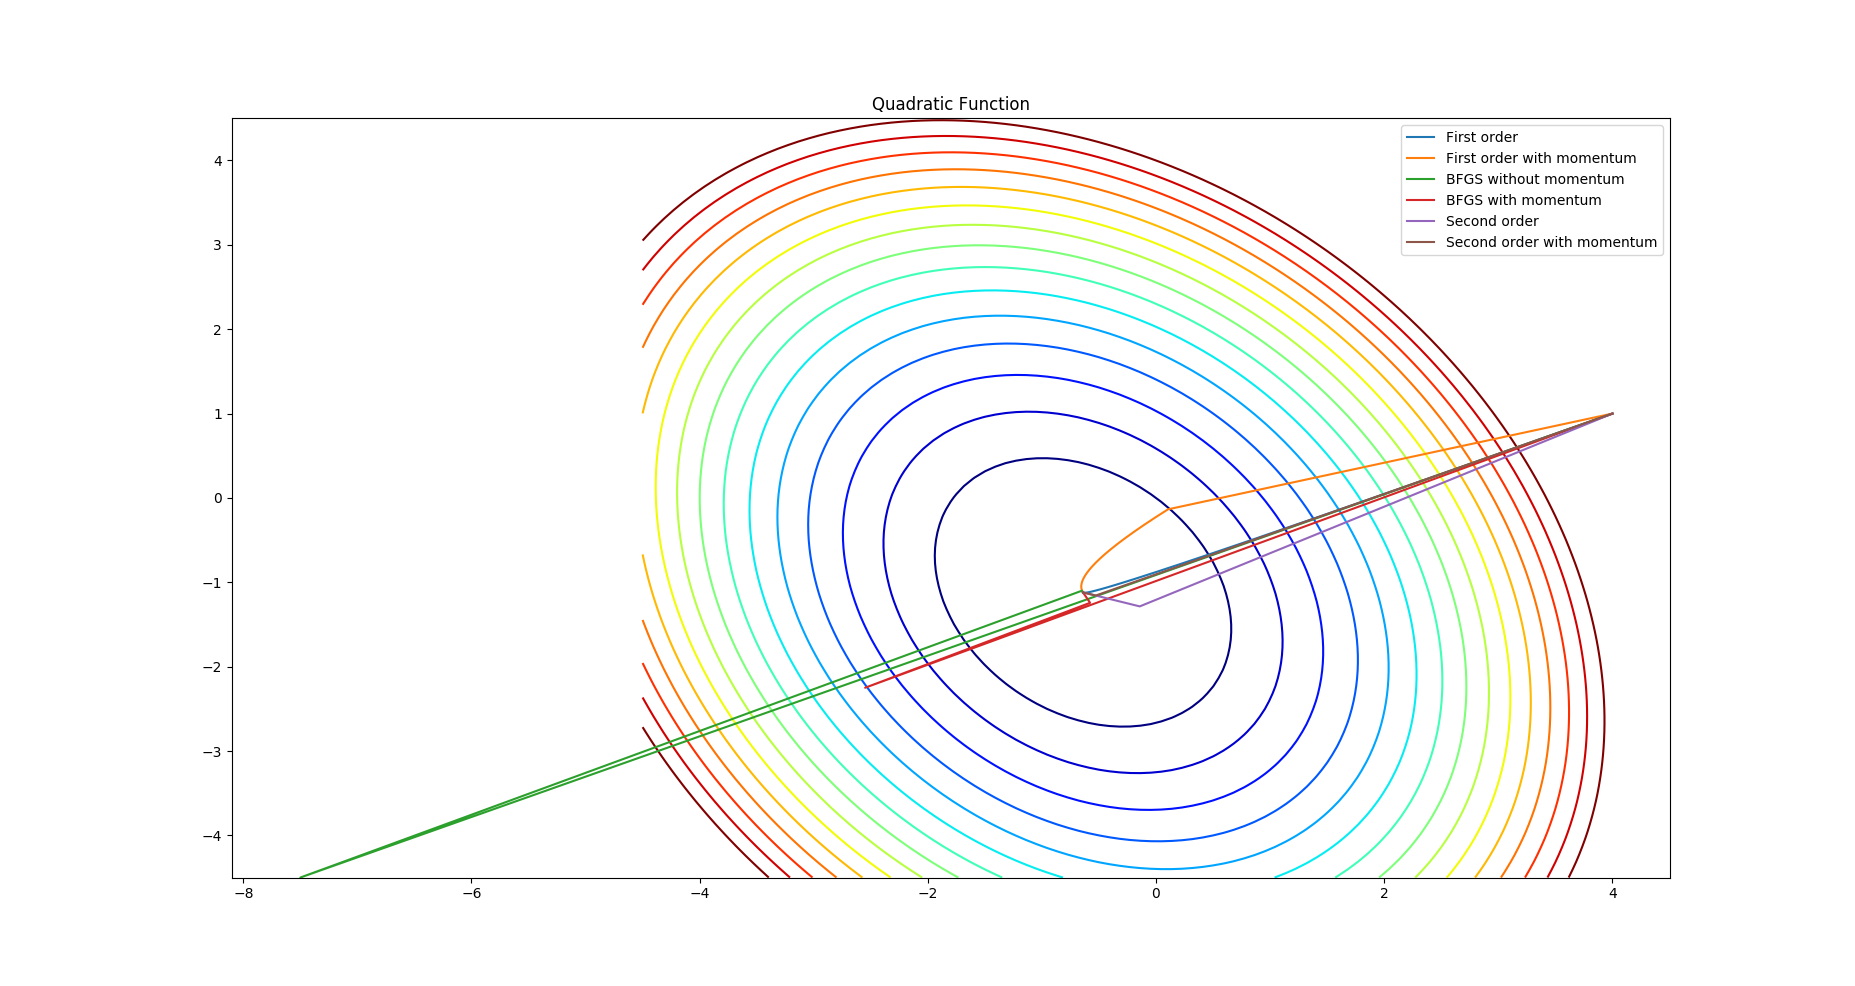
\includegraphics[width=\linewidth]{"/home/vaibhav/P/OMML/Project/Images/quadratic_nesterov.png"}
	\caption{Without Backtracking nesterov momentum}
	\label{fig:Without Backtracking nesterov momentum}
\end{figure}
		
\section{Observations and Inferences}\label{inferences}
<Explain individual tables/graphs here>

Based on our findings, we make the following propositions:

\begin{prop}
	Both momentum and Nesterov's momentum decrease the performance of every method if the the step size is chosen using backtracking line search.
\end{prop}

\begin{prop}
	Both momentum and Nesterov's momentum decrease the performance of Newton's method. 
\end{prop}

\begin{prop}
	Momentum and Nesterov's momentum perform comparable - in some cases better, in some cases worse - than optimization without using them, when used on BFGS.
\end{prop}


\subsection{Limitations}
Our experiments test over a very small set of benchmark functions. It is quite possible that our results and conclusions are biased due to the choice of functions, and that momentum for second order methods performs much better for a different set of functions. However, we believe that this might not be the case, as the functions were chosen with the intent of having as diverse a set of properties among them as possible


\section{Conclusion}\label{conclusion}
Based on our experiments, it appears that momentum degrades the performance of Newton's method. There is no clear advantage on using momentum for BFGS. We also observe that momentum performs poorly, even for gradient descent, when used with backtracking line search.

Momentum for first order methods is based on the intuitive idea of damping gradient descent, which allowed the step sizes to be increased. Over the past many decades, strong convergence guarantees have been proven for using momentum. Nesterov's momentum, proposed in 2013 by \citet{Sutskever}, has performed very well for deep learning. In the case of second order methods, an alternative, more intuitive formulation for acceleration might be required, that can exploit the assumptions made in these methods naturally, as opposed to direct application of the first order formulation.

<Cubic Reg>

http://infinity77.net/global\_optimization/test\_functions.html
http://infinity77.net/global\_optimization/test\_functions.html
http://infinity77.net/global\_optimization/test\_functions.html
\bibliographystyle{unsrtnat}
\bibliography{references}

\end{document}
